\documentclass[a4paper,8pt]{article}
\pagestyle{plain}

\usepackage[utf8]{inputenc}
\usepackage{fancyhdr}
\usepackage[margin=2cm,foot=1cm]{geometry}
\usepackage[T1]{fontenc}
\usepackage{hyperref}
\usepackage{ragged2e}
\usepackage{amsbsy}
\usepackage{xparse}
\usepackage{natbib}
\bibliographystyle{named}

\hypersetup{
	colorlinks,
	linkcolor={blue!80!black},
	citecolor={green!80!black},
	urlcolor={red!80!black}
}

\usepackage[nodisplayskipstretch]{setspace}
\setstretch{1}

% Used to set numbering of the content
\setcounter{tocdepth}{3}
\setcounter{secnumdepth}{3}

\newcommand{\matr}[1]{\mathbf{#1}} % undergraduate algebra version
%\newcommand{\matr}[1]{#1}          % pure math version
%\newcommand{\matr}[1]{\bm{#1}}     % ISO complying version
\newcommand{\vect}[1]{\bm{#1}} % undergraduate algebra version

%%
% Math packages
\usepackage[utf8]{inputenc}
\usepackage{mathtools}
\usepackage{amssymb}
\usepackage{bm}
\usepackage{amsthm}
\usepackage{amsmath}
\usepackage{rotating}
\usepackage{mathrsfs}
\usepackage{tikz-cd}
\usepackage{float}
\usepackage{enumitem}
\usepackage{makecell}

\graphicspath{ {./images/} }

%%
% Math Commands
\def\upint{\mathchoice%
	{\mkern13mu\overline{\vphantom{\intop}\mkern7mu}\mkern-20mu}%
	{\mkern7mu\overline{\vphantom{\intop}\mkern7mu}\mkern-14mu}%
	{\mkern7mu\overline{\vphantom{\intop}\mkern7mu}\mkern-14mu}%
	{\mkern7mu\overline{\vphantom{\intop}\mkern7mu}\mkern-14mu}%
	\int}
\def\lowint{\mkern3mu\underline{\vphantom{\intop}\mkern7mu}\mkern-10mu\int}
\usepackage{tikz}
\newcommand{\N}{\mathbb{N}}
\newcommand{\R}{\mathbb{R}}
\newcommand{\Q}{\mathbb{Q}}
\newcommand{\C}{\mathbb{C}}
\newcommand{\x}{\mathbf{x}}
\newcommand{\F}{\mathbf{F}}
\newcommand{\f}{\mathbf{f}}
\newcommand{\y}{\mathbf{y}}
\renewcommand{\b}{\mathbf{b}}
\renewcommand{\c}{\mathbf{c}}
\renewcommand{\a}{\mathbf{a}}
\newcommand{\h}{\mathbf{h}}
\newcommand{\g}{\mathbf{g}}
\newcommand{\z}{\mathbf{z}}
\newcommand{\ze}{\mathbf{0}}
\newcommand{\Z}{\mathbb{Z}}
\newcommand{\norm}[1]{\left\lVert#1\right\rVert}
\newcommand{\abs}[1]{\left\lvert#1\right\rvert}
\newcommand{\brk}[1]{ \left[#1\right] }
\newcommand{\brc}[1]{ \left\{#1\right\} }
\newcommand{\paren}[1]{ \left(#1\right) }
\newcommand{\normop}[1]{\left\lVert#1\right\rVert_\text{op}}
\newcommand{\LL}{\mathcal{L}}
\newcommand{\uni}{\overset{\text{uni}}{\to}}
\DeclareMathOperator{\diam}{diam}
\newcommand{\Prr}[1]{\text{Pr}\left(#1\right)}
\newcommand{\ceil}[1]{\lceil #1 \rceil}
\newcommand{\floor}[1]{\lfloor #1 \rfloor}

\definecolor{dartmouthgreen}{rgb}{0.05, 0.5, 0.06}
\definecolor{egyptianblue}{rgb}{0.06, 0.2, 0.65}
\definecolor{dukeblue}{rgb}{0.0, 0.0, 0.61}
\definecolor{jazzberryjam}{rgb}{0.65, 0.04, 0.37}
\definecolor{magenta}{HTML}{EC008C}
\definecolor{darkmagenta}{rgb}{0.55, 0.0, 0.55}
\definecolor{deeppink}{rgb}{1.0, 0.08, 0.58}

\newcommand\disteq{\stackrel{\textnormal{dist}}{=}}

\NewDocumentCommand{\evalat}{sO{\big}mm}{%
  \IfBooleanTF{#1}
   {\mleft. #3 \mright|_{#4}}
   {#3#2|_{#4}}%
}

%%
% Self-defined useful shortcuts
\newcommand{\isomorp}{\xrightarrow{\sim}}
\newcommand{\hlt}[1]{\textit{{\color{blue}#1}}}
\newcommand{\simpt}[1]{\textit{{\color{deeppink}#1}}}
\newcommand{\impt}[1]{\textit{{\color{red}#1}}}
\newcommand{\gcds}[1]{\textnormal{gcd}#1}
\newcommand{\mins}[1]{\textnormal{min}#1}
\newcommand{\maxs}[1]{\textnormal{max}#1}
\newcommand{\lcms}[1]{\textnormal{lcm}#1}
\newcommand{\degs}[1]{\textnormal{deg}#1}
\newcommand{\exps}[1]{\textnormal{exp}#1}
\newcommand{\tors}[1]{\textnormal{Tor}#1}
\newcommand{\homs}[1]{\textnormal{Hom}#1}
\newcommand{\anns}[1]{\textnormal{Ann}#1}
\DeclareMathOperator{\sign}{sign}

%%
\setcounter{section}{0}
% Set up math tools
\theoremstyle{theorem}
\newtheorem{theorem}{Theorem}[subsection]
\newtheorem{corollary}[theorem]{Corollary}
\newtheorem{lemma}[theorem]{Lemma}
\newtheorem{proposition}[theorem]{Proposition}
\newtheorem{qnbank}[theorem]{Question Bank}
\let\oldqnbank\qnbank
\renewcommand{\qnbank}{\oldqnbank\normalfont}
\newtheorem{algorithm}[theorem]{Algorithm}
\let\oldalgorithm\algorithm
\renewcommand{\algorithm}{\oldalgorithm\normalfont}
\newtheorem{process}[theorem]{Process}
\let\oldprocess\process
\renewcommand{\process}{\oldprocess\normalfont}
\newtheorem{method}[theorem]{Method}
\let\oldmethod\method
\renewcommand{\method}{\oldmethod\normalfont}
\newtheorem{definition}[theorem]{Definition}
\let\olddefinition\definition
\renewcommand{\definition}{\olddefinition\normalfont}
\newtheorem{example}[theorem]{Example}
\let\oldexample\example
\renewcommand{\example}{\oldexample\normalfont}
\newtheorem{remark}[theorem]{Remark}
\let\oldremark\remark
\renewcommand{\remark}{\oldremark\normalfont}


\title{Algorithmic Trading}
\author{Arthur Li}

\begin{document}
\maketitle
\bibliographystyle{chicago}

\newpage

\tableofcontents

\newpage

\section{Fundamentals of Systematic Trading}

Based on the book by Rishi K. \cite{rishi_2013}, and the book by Raja \cite{velu_2020}.

\subsection{Market Fundmantals}

The basic function of a market is to bring buyers and sellers together.

\begin{process}
\hlt{(Four Components of a Trade)}
\begin{enumerate}[label=\roman*.]
\setlength{\itemsep}{0pt}
\item Acquisition of information and quotes
\begin{enumerate}[label=\arabic*.]
\setlength{\itemsep}{0pt}
\item Quality information and transparency are crucial to price discovery
\item Transparent markets quickly disseminate high-quality information
\item Opaque markets are those that lack transparency
\end{enumerate}
\item Routing of the trade order
\begin{enumerate}[label=\arabic*.]
\setlength{\itemsep}{0pt}
\item Selecting the brokers to handle the trades
\item Deciding which markets will execute the trades and transmitting the trades to the markets
\end{enumerate}
\item Execution. Buys are matched and executed against sells according to the rules of the market
\item Confirmation, clearance and settlement
\begin{enumerate}[label=\arabic*.]
\setlength{\itemsep}{0pt}
\item Clearance is the recording and comparison of the trade records
\item Settlement involves the actual delivery of the security and its payment
\item Might include trade allocation
\end{enumerate}
\end{enumerate}
\end{process}

\begin{remark}
\hlt{(Risks of Algorithmic Trading)}
\begin{enumerate}[label=\roman*.]
\setlength{\itemsep}{0pt}
\item Leaks might arise from competitor efforts to revere engineer them
\item Many algorithms lack the capacity to handle or respond to exceptional or rare events.
\end{enumerate}
\end{remark}

\begin{remark}
\hlt{(Cornering-the-Market)} Trader takes huge long futures position and tries to exercise control over supply of underlying commodity. As maturity of futures contract is approaching, position is not closed, number of outstanding contracts exceed commodities available. Holders of short positions desperately try to close positions, leading to rise in both futures and spot prices.\\
Abuse is dealt with by increasing margin requirements or imposing stricter position limits or prohibiting trades that increase speculator's open position or requiring market participants to close their positions.
\end{remark}

\subsubsection{Liquidity Access in Equity Markets}

\hlt{(Exchanges)} Account for $60\%$ to $70\%$ of all activity. The full order-book, arrivals/cancellations are all published, the liquidity information is transparent. Larger orders may impact the market. Liquidity at best price cannot be ignored, as the exchange will need to reroute to other exchanges where price is better while charging a fee (National Best Bid Offer, NBBO). All exchanges have almost exactly the same trading mechanism, and behave exactly the same way during the trading day except for opening and closing auctions.\\
Most exchanges use maker-taker fee model, but some exchanges (BYX, EDGA, NSX, BX) have an inverted fee model where rebate is provided for taking liquidity. IEX uses a speed bump to remove speed advantages of HFTs, providing a less 'toxic' liquidity pool.\\

\hlt{(Dark Pools/ATS)} Dark pools do not display any order information and use the NBBO as reference price. To avoid accessing protected venues, these pools trade only at the inside market (at or within the bid ask spread). Still possible to identify large blocks of liquidity by 'pinging' the pool at minimum lot size; counteracted by sending orders with minimum fill quantity tag, which allows block to be transparent from small pinging.\\
Most of ATS are run by major investment banks; some venues allow direct trading between investment firms. Note that many of the trading strategies used by firms tend to be highly correlated, hence liquidity is often on the same side; venues have to leverage sell side broker's liquidity to supplement their own.\\

\hlt{(Single Dealer's Platform/Systematic Internalisers)} Broker/Dealer and other institutional clients connect to Single Dealer Platform (SDP) directly. Not regulated ATS, hence can offer unique products. Brokers provide their own SDPs to expose their internal liquidity.\\

\hlt{(Auctions)} Exchanges begin and end day with a primary auction procedure that leverages special order types to accumulate supply and demand, then run algorithm that determines best price that would at best pair off the most volume. An opportunity for active and passive investors to exchange large amounts of liquidity.

\subsubsection{Trading Mechanisms}

Most common approach by modern electronic exchanges is the time/price priority, \hlt{continuous double auction} trading system. There are multiple buyers and multiple sellers participating at the same time.\\

\hlt{(Limit Order Book, LOB)} Stores all non-executed orders with associated instructions. Highly efficient, able to handle a high degree of concurrency to ensure the state is always correct. Has 2 copies of core data structure (for Buy, Sell orders). Supports 3 basic instruction types (insert, cancel, amend). There are 4 events on both Buy and Sell that may alter state of order book (limit order submission, limit order cancellation, limit order amendment, execution).\\

\hlt{(Matching Algorithm)} Responsible for interpreting various events to determine if any buy and sell orders can be matched. When multiple orders can be paired, price/time priority is used, where the order with most competitive prices are matched, and when prices are equal, the order that arrived prior is chosen.\\

Exchanges will publish order imbalance that exists among orders on opening and closing books during \hlt{Open Auctions}, with indicative price and volume. The following are published every second on market data feeds:
\begin{enumerate}[label=\roman*.]
\setlength{\itemsep}{0pt}
\item \hlt{Current Reference Price}: Price at which paired shares are maximised, imbalance is minimised, distance from bid-ask mid-point is minimised, in that order
\item \hlt{Near Indicative Clearing Price}: The crossing price at which orders in opening, closing book and continuous book would clear against each other
\item \hlt{Far Indicative Clearing Price}: The crossing price at which orders in opening, closing book would clear against each other
\item \hlt{Number of Paired Shares}: The number of on-open or on-close shares that is able to pair off at the current reference price
\item \hlt{Imbalance Shares}: The number of opening or closing shares that would remain unexecuted at the current reference price
\item \hlt{Imbalance Side}: The side of imbalance. B is buy-side imbalance; S is sell-side imbalance; N is no imbalance; O is no marketable on-open or on-close orders
\end{enumerate}

In general, the following rules apply to match supply and demand:
\begin{enumerate}[label=\roman*.]
\setlength{\itemsep}{0pt}
\item Crossing price must maximise volume transacted
\item If several prices result in similar volume transacted, the crossing price is the one the closest from last price
\item Cross price is identical for all orders executed
\item If two orders are submitted at same price, the order submitted first has priority
\item It is possible for an order to be partially executed if the other side quantity is not sufficient
\item 'At Market' orders are executed against each other at the determined crossing price, up to available matching quantity on both sides, but generally do not participate in price formation process
\item For Open Auction, unmatched 'At Market' orders are entered into continuous session of LOB as limit orders at the crossing price
\end{enumerate}

The open auction is a major price discovery mechanism, as it occurs after a period of market inactivity when market participants were unable to transact even if they have information. Market participants with better information are more likely to participate, with more aggressive orders to extract liquidity, hence the mechanism is quite volatile and more suited for short-term alpha investors.\\
During execution, smaller orders may avoid participation in open auction and period thereafter; larger orders may participate to extract significant liquidity from the market.\\

Diversity of order types is key component of continuous double auction electronic markets.

\begin{definition} {\color{white}space}
\begin{enumerate}[label=\roman*.]
\setlength{\itemsep}{0pt}
\item \hlt{Market Order}: trade carried out immediately at best price available in market.
\item \hlt{Limit Order}: only executed at this price or at one more favourable to the trader.
\item \hlt{Stop/Stop-Loss Order}: not visible in LOB. Only become active when certain price is reached or passed, then enter order book as ether limit or market order depending on user setup.
\item \hlt{Stop-Limit Order}: combination of stop order and limit order. Order becomes limit order as soon as a bid or ask is made at the price equal to or less favourable than stop price. If stop price and limit price is the same, then the order is \hlt{stop-and-limit} order.
\item \hlt{Trailing Stop Order}: function like stop orders, but stop price is set dynamic rather than static.
\item \hlt{Market-if-Touched (MIT)/Board Order}: executed at best available price after trade occurs at a specified price or more favourable. Ensure profit is taken if sufficiently favourable price movements occur.
\item \hlt{Market-Not-Held/Discretionary Order}: traded as market order, execution may be delayed at broker's discretion for better price.
\item \hlt{All-Or-None Order}: request full execution of order. Not executed until full quantity is available.
\item \hlt{Peg Order}: specify a price level at which order should be continuously and automatically repriced. Used for mid-point executions in non-displayed markets.
\item \hlt{Iceberg Order}: limit order with specific display quantity, designed to prevent information leakage.
\item \hlt{Hidden Order}: when available to trade, not directly available to other market participants in central LOB
\item \hlt{On-Open}: request execution at open price. Can be limit-on-open or market-on-open.
\item \hlt{On-Close}: request execution at close price. Can be limit-on-close or market-on-close.
\item \hlt{Imbalance Only}: provide liquidity intended to offset on-open/on-close order imbalances during opening/closing cross. These generally are limit orders.
\item \hlt{D-Quote}: Special order on NYSE, mainly used during close auction period.
\item \hlt{Funari}: Special order on Tokyo Stock Exchange, allows limit order placed in book during continuous session to automatically enter closing auction as market orders.
\end{enumerate}
\end{definition}

Instruction validity may take the following forms:
\begin{enumerate}[label=\roman*.]
\setlength{\itemsep}{0pt}
\item \hlt{Day Order}: valid for full duration of trading session
\item \hlt{Extended Day Orders}: allows for trading in extended hours
\item \hlt{Good-Till-Cancel Order}: in effect until executed or until end of trading in particular contract
\item \hlt{Immediate-or-Cancel Order}: will be immediately cancelled back to sender after reaching matching engine if it does not get immediate fill.
\item \hlt{Fill-or-Kill Order}: must be executed immediately on receipt or none at all.
\end{enumerate}

\subsubsection{Data Taxonomy}

Data availability, storage, management, and cleaning are the core of any research environment.\\

Reliable \hlt{reference data} is key foundation of a robust quantitative strategy development, with following data:
\begin{enumerate}[label=\roman*.]
\setlength{\itemsep}{0pt}
\item Trading Universe: evolving daily to incorporate new listings, de-listings etc. Knowing when a particular stock no longer trades is important to avoid survivor bias.
\item Symbology Mapping: ISIN, SEDOL, RIC, Bloomberg Tickers etc. Data is not static, symbols may change, complicating historical data merges. Mapping needs to persist as point-in-time data and allow for historical 'as-of-date' usage, require implementation of bi-temporal data structure. 
\item Ticker Changes: for reasons described in symbology mapping. To maintain historical table of ticker changes to seamlessly go up and down time series data.
\item Corporate Actions Calendars: contain stock and cash dividends (announcement, execution date), stock splits, reverse splits, rights offer, mergers and acquisitions, spin off, free float or shares outstanding adjustments, quotation suspensions etc.\\
For dividends, announcements may coincide with more volatility, jumps in price time series. Allow building of strategies that look to benefit from the added volatility.\\
For stock splits, reverse splits, rights offers, all historical data need to be adjusted backward to reflect the split (both volume and price).\\
For M\&A, spin-offs, to account for changes in valuation, hence used in Merger Arbitrage strategies.\\
Suspensions result in gaps in data, may impact backtesting.
\item Static Data: country, sector, primary exchange, currency, and quote factor. May be used to group instruments based on fundamental similarities (hence for pairs trading). Maintaining a table of quotation currency per instrument necessary to aggregate positions at portfolio level.
\item Exchange Specific Data: individual exchanges have variety of differences to be accounted for when designing trading strategies. First group of information concerns the hours and dates of operations:
\begin{enumerate}[label=\arabic*.]
\setlength{\itemsep}{0pt}
\item Holiday Calendar: Strategies trading simultaneously in several markets and leveraging correlation may not perform as well if one market is closed and another is open.
\item Exchange Sessions Hours: Different sessions (Pre-Market, Continuous Core, After-Hour etc.); auction times and respective cutoff times for oder submission; lunch break restricting intraday trading and auctions before/after lunch; settlement times for futures market. Daylight Saving Time (DST) adjustments; length of trading hours during course of the year; different trading hours by venue.
\item Disrupted Days: Exchange outages or trading disruptions, market data issues. To be recorded so they can be filtered out when building or testing strategies.
\end{enumerate}
Second group of information governing the mechanics of trading:
\begin{enumerate}[label=\arabic*.]
\setlength{\itemsep}{0pt}
\item Tick Size: Minimum eligible price increment; may vary by instrument and as a function of price.
\item Trade and Quote Lots: Minimum size increment for quotes or trades.
\item Limit-Up and Limit-Down Constraints: Maximum daily fluctuations of securities, and whether trading is paused or can only be traded at better prices than the threshold.
\item Short Sell Restrictions: Restrict shot sells not to trade at price worse than last price, or not to create a new quote that will be lower than the lowest prevailing quote. Impact ability to source liquidity.
\end{enumerate}
\item Market Data Condition Codes: vary per exchange and asset class, and each market event may be attributed to several codes at once. To build mapping table of condition codes and what they mean (i.e., auction trade, lit or dark trade, cancelled or corrected trade, regular trade, off-exchange trade reporting, block-size trade, trade originating from multi-leg order such as option spread trade etc.). To access liquidity for trading algorithm, trades published for reporting purposes must be excluded and not be used to update some of the aggregated daily data used in construction of trading strategies.
\item Special Day Calendars: days wth distinct liquidity characteristics to be accounted for in both execution strategies and in alpha generation process. These (non-exhaustive) irregular events may be:
\begin{enumerate}[label=\arabic*.]
\setlength{\itemsep}{0pt}
\item Half trading days preceding Christmas and following thanksgiving in US
\item Ramandan even in Turkey
\item Taiwan market opening on weekend to make up for lost trading days during holiday periods
\item Korean market changing trading hours on day of nationwide university entrance exam
\item Brazilian market opening late on day following the Carnival
\item Last trading days of months and quarters (investors rebalance portfolios)
\item Index rebalancing dates, where intraday volume distribution is significantly skewed toward EODs
\item Options and futures expiry dates (quarterly/monthly expiry, Triple Witching in US, Special Quotations in Japan) where excess trading volume and different intraday patterns result from hedging activity and portfolio adjustments.
\end{enumerate}
Model normal days first. Special days are modelled either independently, or using normal days as baseline.
\item Futures-Specific Reference Data: to know which contract was live at any point of time by using expiry calendar, and the most liquid contract. Equity index futures are most liquid for first contract available (front month), energy futures such as oil are more liquid for second contract. Hence to know which contract carry the most significant price formation characteristics, and what is true liquidity available.\\
Note there is no real standardised expiry frequency that applies across markets. When computing rolling-window metrics, to account for potential roll dates (due to investors rolling forward positions) that may have happened during the time span. May blend volume time series prior to roll date and after roll date.\\
Futures market also have different market phases during the day with significantly different liquidity characteristics. Various market data metrics (volume profile, average spread, average bid-ask sizes etc) should be computed separately for each market phase by maintaining a table of start and end times of each session for each contract.
\item Options-Specific Reference Data (Options Chain): expiry date and strike price combination (option chain). Map of equity tickers to option tickers with strike and expiry dates allow for design for more complex investment and hedging strategies (i.e., distance to strike, change in open interest of puts and calls).
\item Market-Moving News Releases: macroeconomic announcements. To maintain calendar of dates and times of their occurrences to assess their impact on strategies. Central bank announcements or meeting minutes releases about major economies (FED/FOMC, ECB, BOE, BOJ, SNB), Non-Farm Payrolls, Purchasing Managers' Index, Manufacturing Index, Crude Oil Inventories etc.\\
Stock-specific releases such as earnings calendars, specialised sector events (for healthcare, biotech etc).
\item Related Tickers: tickers that are related to each other as they fundamentally represent the same underlying asset. Allows efficient opportunity exploitation. Primary tickers to composite tickers mapping (for markets with fragmented liquidity), dual listed/fungible securities in US and Canada, ADR or GDR, local and foreign boards in Thailand etc.
\item Composite Assets: ETFs, Indexes, Mutual Funds etc. May be used to achieve desired exposures, or as cheap hedging instruments, and provide arbitrage opportunities when they deviate from NAV. To maintain information such as time series of their constituents and value of any cash component, divisor used to translate NAV into quoted price, constituent weights.
\item Latency tables: for higher frequency trading strategies. Contains distribution of latency between different data centres for more efficient order routing, and reordering data that are recorded in different locations.
\end{enumerate}

There are different details in the \hlt{market data} feed, as follows:
\begin{enumerate}[label=\roman*.]
\setlength{\itemsep}{0pt}
\item Level I Data (Trade and BBO Quotes): trades and top of book quotes. Enough to reconstruct Best Bid and Offer (BBO). Also contains information in form of trade status (cancelled, reported late etc), trade and quote qualifiers (odd lot, normal trade, auction trade, Intermarket Sweep, average price reporting, on which exchange etc). May be used to analyse sequence of events and decide if a given print should be used to update the last price and total volume traded at a point in time.
\item Level II Data (Market Depth): addition of quote depth data, displays all lit limit order book updates (price changes, addition or removal of shares quoted) at any level in the book, for all of the lit venues in fragmented markets.
\item Level III Data (Full Order View): message data. Each order arriving is attributed a unique ID for tracking over time, and is precisely identified when it is executed, cancelled, or amended. Possible to build a full (with national depth) book at any moment intraday. Example from US market:
\begin{enumerate}[label=\arabic*.]
\setlength{\itemsep}{0pt}
\item Timestamp: number of milliseconds after midnight
\item Ticker: equity symbol (up to 8 char)
\item Order: Unique order ID
\item T: message type. 'B' is add buy order; 'S' is add sell order'; 'E' is execute outstanding order in part; 'C' is cancel outstanding order in part; 'F' is execute outstanding order in full; 'D' is delete outstanding order in full; 'X' is bulk volume for cross event; 'T' is execute non-displayed order
\item Shares: order quantity for 'B', 'S', 'E', 'X', 'C', 'T' messages. Zero for 'F', 'D' messages
\item Price: order price for 'B', 'S', 'X', 'T' messages. Zero for cancellation and executions. Last 4 digits are decimal, padded to right with zeroes. Divide by $1000$ to convert to currency value.
\item MPID: Market Participant ID associated with transaction (4 char)
\item MCID: Market Centre Code for originating exchange (1 char)
\end{enumerate}
A few special types of orders worth mentioning are:
\begin{enumerate}[label=\arabic*.]
\setlength{\itemsep}{0pt}
\item Order subject to price sliding: execution price may be one cent worse than display price at NASDAQ; ranked at locking price as hidden order, displayed at the price one minimum price variation inferior to locking price. New order ID will be used if order is replaced as a display order.
\item Pegged order: based on NBBO, not routable, new timestamp given upon repricing; display rule vary over exchanges
\item Mid-point peg order: non-displayed, may result in half-penny execution
\item Reserve order: displayed size is ranked as displayed limit order; reserve size is behind non-displayed orders and pegged orders in priority.\\
Minimum display quantity is 100, amount replenished from reserve size when it falls below 100 shares; New timestamp created, displayed size re-ranked upon replenishment.
\item Discretionary order: displayed at one price while passively trading a more aggressive discretionary price. Order becomes active when shares are available within discretionary price range. Order ranked last in priority. Execution price may be worse than display price.
\item Intermarket sweep order: can be executed without need for checking prevailing NBBO. 
\end{enumerate}
Using these data, we may model: the pattern of inter-arrival times of various events; arrival and cancellation rates as a function of distance from nearest touch price; arrival and cancellation rates as a function of other information, such as in the queue on either side of the book, order book imbalance etc.\\
Once modelled, we may analyse: the impact of market order on limit order book; chances for limit order to move up the queue from given entry position; probability of earning the spread; expected direction of price movement over a short horizon.
\end{enumerate}

Most quantitative strategies rely on \hlt{binned data}, such as the following daily statistics:
\begin{enumerate}[label=\roman*.]
\setlength{\itemsep}{0pt}
\item Open, High, Low, Close (OHLC) and Previous Close Price: indication on trading activity and intraday volatility. Distance traveled between lowest and highest points is indication of market sentiment. Previous close has to be adjusted for corporate actions and dividends.
\item Last Trade before Close (Price/Size/Time): how much the close price may have jumped in final moments of trading; how stable it is as a reference value for next day.
\item Volume: trading activity indicator, especially when level jumps from long term average. Collect volume breakdown between lit and dark venues for execution strategies.
\item Auctions Volume and Price: price discovery event when significant volume prints occur.
\item VWAP: indication of trading activity on the day. Easier to algorithmically execute large orders with VWAP than a single print.
\item Short Interest/Days-to-Cover/Utilisation: good proxy for investor position. Short pressure an indication of upcoming short term moves: large short interest is bearish view from institutional investors. Utilisation level of available securities to borrow gives indication of how much room is left for future shorting. Days-to-Cover to assess magnitude of potential short squeeze (if sellers unwind position, fraction of available daily liquidity needed); larger value indicates larger potential of sudden upswing on heavily shorted securities.
\item Futures Data: insight into activity or large investors through open interest data. Offer arbitrage opportunities if their basis exhibits mis-pricing compared to one's dividend estimates.
\item Index-Level Data: source of relative measures for instrument specific features (index OHLC, volatility). Normalised features identify individual instruments deviating from their benchmarks.
\item Options Data: information on position of traders through open interest and Greeks.
\item Asset Class Specific: yield/benchmark rates (repo, 2y, 10y, 30y), CDS spreads, US Dollar Index
\end{enumerate}
We also consider data for granular intraday microstructure activity:
\begin{enumerate}[label=\roman*.]
\setlength{\itemsep}{0pt}
\item Number and Frequency of Trades: proxy for activity level, and how continuous it is. Low number of trades mean harder execution, and may be more volatile
\item Number and Frequency of Quote Updates: similar proxy for activity level
\item Top of Book Size; proxy for liquidity of instruments (larger top of book size makes it possible to trade larger order quasi immediately)
\item Depth of Book (price and size): similar proxy for liquidity
\item Spread Size (average, median, time weighted average): proxy for cost of trading. Parametrised distribution used to identify opportunities if they are cheap or expensive
\item Trade size (average, median): to identify intraday liquidity opportunities when examining volume available in the order book.
\item Ticking time (average, median): representation of how often one should expect changes in the order book first level. For execution algorithms for which the frequency of updates (adding/cancelling child orders, re-evaluating decisions etc.) should commensurate with characteristics of the traded instrument.
\end{enumerate}
Daily distribution of these intraday variables can be used as start of day estimates and updated intraday with online Bayesian updates.\\
Last group of daily data is derived from previous two groups but stored pre-computed to save time during research phase, or to be used as normalising values:
\begin{enumerate}[label=\roman*.]
\setlength{\itemsep}{0pt}
\item X-day Average Daily Volume (ADV) / Average Auction Volume
\item X-day Volatility (close-to-close, open-to-close etc)
\item Beta with respect to index or sector (plain beta, or asymmetric up-days/down-days beta)
\item Correlation matrix
\end{enumerate}

When binning data, this may be grouped into bins ranging from a few seconds to 30 minutes. Minute bar data are used for volume and spread profiles to prevent introducing excess noise due to market friction.\\

Some \hlt{fundamental data} and other data sets which may be considered are as follows:
\begin{enumerate}[label=\roman*.]
\setlength{\itemsep}{0pt}
\item Key Ratios: Earnings Per Share (EPS), Price-to-Earning (P/E), Price-to-Book (P/B), etc. 
\item Analyst Recommendations: aggregated values given consensus valuation
\item Earnings data: estimations by research analysts provide quarterly earning estimates which can be used as indication of performance of stock before actual value is published
\item Holders: sudden changes in ownership indicate changes in sentiment by sophisticated investor
\item Insiders Purchase/Sale: indicator of future stock price moves from group of people who have access to best possible information about the company
\item Credit Ratings: credit downgrades resulting in higher funding costs in the future have negative impact on equity prices
\end{enumerate}

\subsubsection{Market Microstructure Primer}

A market microstructure analysis framework follows three main categories:
\begin{enumerate}[label=\roman*.]
\setlength{\itemsep}{0pt}
\item Price Formation and Price Discover: how prices impound information over time, and how determinants of trading costs vary
\item Market Design: impact of trading rules on price formation. Choice of tick size, circuit breakers that halt trading in event of large price swings, degree of anonymity, transparency of information to market participants. These create a diverse set of constraints and opportunities.
\item Transparency: quantity, quality and speed of information effect on trading process. Classified into pre-trade (lit order book), post-trade (trade reporting to public). 
\end{enumerate}

Topics for research in microstructure includes the following:
\begin{enumerate}[label=\roman*.]
\setlength{\itemsep}{0pt}
\item Parent order sliced into several child orders sent to market for execution; difficult to discern the informed trader who use sophisticated dynamic algorithms. Retail trades usually cross the spread.
\item Understanding of trading intensity in short intervals. Order imbalance is empirically shown to be unrelated to price levels.
\item Informed traders usage of hidden orders in entering and exiting the market require further studies.
\item Traders respond to changing market conditions by revising quoted prices. Quote volatility can provide valuable information about perceived uncertainty in the market.
\end{enumerate}


\newpage

\subsection{Mathematical Primer: Basic Models}

A review of some basic and advanced statistical methodologies that are useful for developing trading strategies.

\subsubsection{Univariate Time Series Models}

Trading activities through an exchange can be described by a sequence of time stamps ('ticks') $t_0 < t_1 < \cdots < t_n$, and 'marks' $y_i$ at time $t_i$, where $t_i$ denote market open, $t_n$ denote market close. The marks $y_i$ is a characteristic of the order book at time of $i$th activity. Events with marks associated with the ticks can be described mathematically as a marked point process.
\begin{figure}[H]
\centering
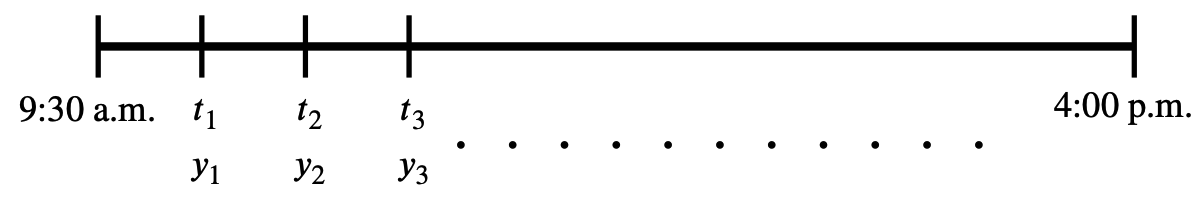
\includegraphics[scale=0.4]{/fundamentals/ticksandmarks}
\caption{Ticks and Marks}
\end{figure}

A data aggregation method is where aggregation is conducted when there is a change in marker. An alternative aggregation method would be to divide the time span $T$ for exchange hours into $K$ intervals, so regularly spaced intervals are of size $\Delta t = T/K$. The time series method to be discussed will apply to all aggregated data.\\

Let $p_{it} = \ln P_{it}$ denote price of $i$th asset at time $t$; $p_t = (p_{1t}, p_{2t}, \ldots, p_{nt})$ denote price vector for $n$ assets; $y_{it}$ denote vector of characteristics of $i$th asset at time $t$. These quantities are aggregated from high frequency data. Consider $r$ factors $f_t = (f_{1t}, f_{2t}, \ldots, f_{rt})$ that may include market and industry factors, and asset characteristics. Trading rules can be broadly grouped as follows:
\begin{enumerate}[label=\roman*.]
\setlength{\itemsep}{0pt}
\item \hlt{Statistical Arbitrage}: $E(p_{i, t+1} \ \vert \ p_{i,t}, p_{i, t-1}, \ldots, y_{i,t}, y_{i, t-1}, \ldots)$, that predicts the price of $i$th stock at $t+1$ based on past trading information (also known as time series momentum)
\item \hlt{Momentum}: $E(p_{t+1} \ \vert \ p_t, p_{t-1}, \ldots, y_t, y_{t-1}, \ldots)$, that predicts the cross-sectional momentum of a subset of stocks based on past trading characteristics. For portfolio formation and rebalancing, pairs trading
\item \hlt{Fair Value}: $E(p_{t+1} \ \vert \ p_{t}, p_{t-1}, \ldots, y_t, y_{t-1}, \ldots, f_t, f_{t-1}, \ldots)$, predicts price using all relevant quantities. Factors normally include market, Fama-French; at a more macro level than timescale considered for price prediction, but may still be useful.
\end{enumerate}

Hence price and volatility prediction can be formulated as a tie series prediction problem. Autocorrelations and partial autocorrelations can be used to build autoregressive and ARCH models with some predictive power.




\newpage

\subsubsection{Alpha models}

Theory-driven models tests theories of why markets behave in a manner, and see if they can be used to predict the future. Strategies utilising price-related data are trend and mean reversion; strategies utilising fundamental data are value/yield, growth and quality. Usually more than one model is used in combination.

\begin{definition} \hlt{Theory Driven Models}
\begin{enumerate}[label=\roman*.]
\setlength{\itemsep}{0pt}
\item Trend Following: markets move in given direction long enough that the trend can be identified. As more data support the bull/bear thesis in an uncertain market, more market participants will adopt the same thesis and hence move the asset price to a new equilibrium.\\
Moving average crossover indicator strategy has less than one point of return for every point of downside risk taken, as market behaviour are unstable and episodic.
\item Mean Reversion: markets move in opposite direction to the prevailing trend. Short-term imbalances between buyers and sellers due to liquidity forces prices to move abruptly in one direction, which increases probability of trend reversion as liquidity issue is resolved.\\
Statistical arbitrage bets on convergence of prices of similar stocks whose prices have diverged.\\
Longer-term trends can occur despite smaller oscillations around these trends occurring in the shorter term, hence both strategies may be used in conjunction.
\item Value/Yield:  value strategies uses ratios of fundamental factor against the price of the instrument, inverted to keep the ratio consistent. The higher the yield, the cheaper the instrument.\\
Buying undervalued security and selling overvalued security is a \hlt{carry trade}. The difference between yield received and yield paid is the \hlt{carry}.\\
\hlt{Quant Long Short (QLS)} ranks stocks by attractiveness based on various factors such as value, then buy the higher-ranked stocks while shorting the lower-ranked stocks.
\item Growth: make predictions based on asset's expected or historically observed level of economic growth. Forward-looking growth expectations are typically used as a metric.\\
Growth is trending, and strongest growers are becoming more dominant relative to competitors. Macro growth factors may be used on foreign exchange, while micro growth factors may be used on companies.
\item Quality: All else being equal, it is better to long high quality and short low quality. Capital safety is important. Factors include earnings quality, equity-to-debt ratios etc.
\end{enumerate}
\end{definition}

Data-driven models are more difficult to understand, with more complicated mathematics. Relies on data mining, more technically challenging and far less widely practiced. Typically more used in high-frequency space, as they can discern how market behaves without caring about the economic theory or rational.

\begin{method} \hlt{Strategy Parameters}\\
An implementation approach requires a forecast target, time horizon, bet structure, investment universe, model specification, and run frequency.
\begin{enumerate}[label=\roman*.]
\setlength{\itemsep}{0pt}
\item Forecast Target: models may forecast direction, magnitude, duration of move, and may include probability into the forecast. Signal strength is of importance, defined by a larger expected return and/or higher likelihood of return. A higher level of signal strength results in a bigger bet taken on the position.
\item Time Horizon: models may have forecast horizons ranging from microseconds to years. There are more variability between short-term and long-term strategies, as short-term strategies are making very large number of trades compared to long-term strategies.
\item Bet Structure: models can be made to forecast an instrument relative in itself or to others. For relative forecasts, smaller clusters (pairs) or larger clusters (sectors) may be used. For pairs, few assets can be compared precisely and directly. Large cluster grouping may eliminate impact of general movement of the sector and hence focus on the relative movement of stocks within the sector, allowing for clearer distinction between group behaviour and idiosyncratic behaviour. Clusters may be created either via statistical methods or using heuristics (i.e., fundamentally defined industry groups).\\
Statistical methods may be fooled by data, leading to bad grouping. Heuristic grouping may be imprecise for conglomerates, and may be too rigid. Relative alpha strategies tend to exhibit smoother returns during normal times than intrinsic alpha strategies, but may face incorrect groupings during stressful periods. This may be mitigated by utilising several grouping techniques in concert.
\item Investment Universe: choices made on geography, asset class, instrument class, and exclusions. Liquidity is preferred so estimations of transaction costs are reliable. Large quantities of high quality data is required, which is found in highly liquid and developed markets. Instruments with consistent behaviour is preferred, hence biotech stocks are excluded due to sudden, violent price changes. Hence, the most common asset classes and instruments modelled are common stocks, futures (on bonds and equity indices) and forex.
\item Model Specification: focuses on definition of the strategy mathematically, and may be the source of alpha. Specification details in terms of machine learning or data mining techniques are also defined, to assist in fitting models to the data and setting parameter values. Refitting frequency is also defined to refresh the model and make it adapt to current market conditions; may lead to greater risk of overfitting.
\item Run Frequency: defined from monthly to real time frequency. Increasing frequency of runs lead to greater number of transactions and hence higher transaction costs, and risk of moving portfolio based on noisy data. Less frequency of runs lead to smaller number of larger-sized trades, hence may move the market with block trades; may also miss opportunities to trade at more favourable prices.
\end{enumerate}
\end{method}

\begin{method} \hlt{Blending of Models}\\
Most common approaches are linear models, nonlinear models, and machine learning models. If models are not combined, then several portfolios are constructed based on output from each model, then combined using portfolio construction techniques. The best method depends on the model.
\begin{enumerate}[label=\roman*.]
\setlength{\itemsep}{0pt}
\item Linear Models: require independence of factors, and each factor to be additive. To determine the weight of each alpha factor, multiple regression techniques may be used.
\item Nonlinear Models: used when factors are not independent, or the relationship changes over time. Conditional models base the weight of one factor on the reading of another factor. Rotational models assign weights of factors that fluctuate over time based on updated calculations of the various signal's weights, giving higher weights to factors with better performance recently.
\item Machine Learning Models: developing machine learning strategies takes as much effort to produce one true investment strategy as to produce a hundred. The complexities include data curation and processing, HPC infrastructure, software development, feature analysis, execution simulations, backtesting etc.\\
Decades ago, macroscopic alpha based on simple tools like econometrics are common, but this is quickly diminishing. Microscopic alpha however, becomes more abundant, but requires heavy ML tools.
\end{enumerate}
\end{method}


\newpage

\subsubsection{Risk Models}

Risk models are indispensable tools in algorithmic trading, providing a quantitative framework to assess, monitor, and manage the inherent risks of financial markets. They not only serve to measure exposure but also guide portfolio construction, hedging strategies, and overall risk control.

\begin{method} \hlt{Factor-Based Models}\\
Factor-based models decompose asset returns into contributions from systematic factors and idiosyncratic components. The most common factors include:
\begin{enumerate}[label=\roman*.]
	\setlength{\itemsep}{0pt}
    \item \textbf{Market Factor:} Captures the overall movement of the market.
    \item \textbf{Size Factor:} Reflects the differential risk associated with companies of varying market capitalizations.
    \item \textbf{Value Factor:} Accounts for risk due to discrepancies between market prices and fundamental valuations.
    \item \textbf{Momentum Factor:} Measures the tendency of asset prices to continue in their current trajectory.
\end{enumerate}
This allows traders to understand which elements drive portfolio risk and adjust exposures accordingly.
\end{method}

\begin{method} \hlt{Statistical Models}\\
Statistical risk models leverage historical data and probabilistic techniques to quantify risk parameters.
\begin{enumerate}[label=\roman*.]
	\setlength{\itemsep}{0pt}
    \item \textbf{Historical Simulation:} Directly computing risk metrics from past return distributions.
    \item \textbf{Monte Carlo Simulation:} Generating a large number of potential future return scenarios to estimate risk under diverse conditions.
    \item \textbf{Parametric Methods:} Employing analytical formulas based on assumed return distributions to calculate key risk measures.
\end{enumerate}
These are useful for dynamically updating risk assessments as new market data become available.
\end{method}

\begin{method} \hlt{Limiting Size of Risk}\\
Quantitative risk models are designed to limit the size of exposures to enhance return consistency.
\begin{enumerate}[label=\roman*.]
	\setlength{\itemsep}{0pt}
    \item \textbf{Constraint Mechanisms:}
        \begin{enumerate}[label=\alph*.]
            \item \textbf{Hard Constraints:} Absolute limits imposed on position sizes, which may be set arbitrarily.
            \item \textbf{Penalty Functions:} Flexible constraints where positions can exceed the limit if the alpha model forecasts significantly higher returns, with penalties applied for surpassing the prescribed levels.
        \end{enumerate}
    \item \textbf{Risk Measurement Approaches:}
        \begin{enumerate}[label=\alph*.]
            \item \textbf{Longitudinal Analysis:} Evaluates risk by assessing the volatility of an instrument over time.
            \item \textbf{Dispersion Analysis:} Measures risk by analyzing the correlation or covariance between assets.
        \end{enumerate}
\end{enumerate}
These methods can be applied to single positions, groups of positions (such as sectors or asset classes), different types of risk exposures, and overall portfolio leverage.
\end{method}

\begin{method} \hlt{Limiting the Types of Risk}\\
To eliminate unintentional exposure as there is no expectation of being compensated sufficiently for accepting them. This can be achieved the following measures:
\begin{enumerate}[label=\roman*.]
	\setlength{\itemsep}{0pt}
    \item \textbf{Market Exposure Restriction:} Focus on specific market segments to avoid undue exposure to volatile or unpredictable markets.
    \item \textbf{Leverage Management:} Limit the use of leverage by enforcing conservative leverage ratios to mitigate amplified losses.
    \item \textbf{Stop-Loss Policies:} Implement strict stop-loss rules to automatically exit positions that breach predetermined loss thresholds.
    \item \textbf{Position Size Controls:} Cap individual position sizes relative to overall portfolio risk, ensuring no single trade unduly influences portfolio performance.
    \item \textbf{Regular Risk Assessments:} Continuously monitor risk metrics and adjust risk parameters to reflect evolving market conditions.
\end{enumerate}
\end{method}


\newpage

\subsubsection{Transaction Cost Models}

A trade is executed only if it improves the probability or magnitude of a return (as predicted by alpha model) or reduces likelihood or extent of a loss (as determined by risk model). However, this improvement must be greater than cost of trading. Note that transaction cost model is intended not to minimize trading costs directly, but rather to inform the portfolio construction engine of the costs associated with executing a given trade.

\begin{remark} \hlt{Transaction Cost Components}
\begin{enumerate}[label=\roman*.]
\setlength{\itemsep}{0pt}
    \item \textbf{Commissions and Fees:} These are payments made to brokerages (for accessing other market participants), exchanges (for enhanced transaction security), and regulators (for maintaining operational infrastructure). In the context of quantitative trading, where bank infrastructure is utilized, brokerage commissions tend to be minimal on a per-trade basis.\\[1mm]
    Brokers also charge clearing and settlement fees. \emph{Clearing} involves activities such as regulatory reporting and monitoring, tax handling, and failure management, all of which occur before settlement. \emph{Settlement} is the final delivery of securities in exchange for full payment.
    \item \textbf{Slippage:} This refers to the change in price between the moment the trading system decides to execute a transaction and the time the order is actually sent to the exchange. Trend-following strategies tend to experience more slippage because the assets are already moving in the desired direction, whereas mean-reverting strategies are less affected. Reduced latency to market minimizes slippage, while higher asset volatility increases it.  
    \item \textbf{Market Impact:} This measures the extent to which an order influences the market through its demand for liquidity. The market impact remains uncertain until after the trade is executed. Additionally, there can be an interaction between slippage and market impact (i.e., selling during an upward trending market).
\end{enumerate}
\end{remark}

\begin{definition} \hlt{Types of Transaction Cost Models}
\begin{enumerate}[label=\roman*.]
\setlength{\itemsep}{0pt}
    \item \textbf{Flat Model:} Assumes that the cost of trading remains constant regardless of the order size. This model is appropriate when the traded size is nearly uniform and liquidity remains stable.
    \item \textbf{Linear Model:} In this model, the trading cost increases at a constant rate relative to the order size. It provides a better estimate than the flat model.  
    \item \textbf{Piece-Wise Linear Model:} This approach employs piece-wise linear functions to model costs. It strikes a balance between simplicity and accuracy, offering improved precision compared to flat or linear models.
    \item \textbf{Quadratic Model:} Although the most computationally intensive, the quadratic model delivers the highest accuracy in cost estimation.
\end{enumerate}
\end{definition}


\newpage

\subsubsection{Portfolio Construction Models}

Comes in two major forms: rule-based, optimisers. Rule-based models are based on heuristics, can be exceedingly simple or rather complex, and derived from human experience (trial and error). Optimisers comprises of an objective function and uses algorithms to reach the end goal.

\begin{definition} \hlt{Rule-Based Models}
\begin{enumerate}[label=\roman*.]
\setlength{\itemsep}{0pt}
\item Equal Position Weighting: used if portfolio manager believes that if a position is good enough to own, no other information is needed in determining its size. Strength of signal is not used as input in weighting.\\
Model assumes that there is sufficient statistical strength and power to predict not only direction but also magnitude relative to other forecasts in the portfolio. Portfolio takes few large bets on 'best' forecast, many smaller bets on less dramatic forecasts; may take excess risk in an idiosyncratic event on a seemingly attractive position, resulting in adverse selection bias.
\item Equal Risk Weighting: adjust position sizes inversely to volatilities or a measure of risk. More volatile positions given smaller allocations, less volatile positions given larger allocations.\\
When unit of risk is equalised, it is almost always a backward-looking measurement such as volatility. If volatility changes with time, then model will be misled.
\item Alpha-Driven Weighting: position size based primarily on alpha model. Alpha signal determines size of position, but usually with size limits. Constraints used also includes limits on size of total bet on a group. May also have a function that relates the magnitude of forecast to size of position.\\
If model used in futures trend following, might suffer sharp drawdowns. Reliance on accuracy of alpha.
\item Decision-Tree Weighting: decision path to arrive at the allocation for given instrument, depending on type of alpha model and type of instrument. Constraints may include percentage limits for allocation.\\
Model size grows dramatically if more alpha models or mode types of positions are included.
\end{enumerate}
\end{definition}

\begin{remark} \hlt{Optimisers Models Parameters}\\
Harry Markowitz's mean variance optimisation (MVO) as the pioneer model. Models are based on principles of modern portfolio theory (MPT). Inputs include asset expected return (mean), asset variance, expected correlation matrix. Other inputs include size of portfolio in currency terms, desired risk level (volatility or expected drawdown), and other constraints such as liquidity, universe limits.\\
Model uses an objective function and an algorithm to seek the goal, usually maximising return of portfolio relative to volatility of portfolio returns.
\begin{enumerate}[label=\roman*.]
\setlength{\itemsep}{0pt}
\item Expected Return: alpha models as basis of expected return, which also includes expected direction.
\item Expected Volatility: stochastic volatility forecasting methods is commonly used, as volatility may have high and low periods, with occasional jumps. GARCH model is most used.
\item Expected Correlation: as instrument correlations are not stable over time, it is more appropriate to group assets together before computing correlation within the group.
\end{enumerate}
\end{remark}

\begin{method} \hlt{Optimisation Techniques}
\begin{enumerate}[label=\roman*.]
\setlength{\itemsep}{0pt}
\item Unconstrained Optimisation: most basic form with no constraints. Might provide a single-instrument portfolio, where all money will be invested in instrument with highest risk-adjusted return.
\item Constrained optimisation: constraints include position limits, limits on various groupings of instruments. Might result in constraints driving the portfolio construction more than the optimiser.
\item Black-Litterman Optimisation: blends investor expectations with a degree of confidence about those expectations, and these with historical precedent evident in the data. Adjusts historically observed correlation levels by utilising investor's forecast of return for the various instruments.
\item Grinold and Kahn's Approach: builds a portfolio of signals, instead of sizing positions. To build factor portfolios, each of which are usually rule-based portfolios based on a single type of alpha forecast. Each portfolio backtested, then series of returns are then treated as instruments of a portfolio by the optimiser.\\
Number of factor portfolios is more manageable, usually not more than 20. What is optimised is then a handful of factor portfolios. The model allows for inclusion of risk model, transaction cost model, portfolio size, and risk targets as inputs.
\item Resampled Efficiency: to improve the inputs to optimisation by addressing oversensitivity to estimation error. To resample data using Monte Carlo simulation to reduce estimation error in inputs to the optimiser.
\item Data-Mining Approaches: machine learning techniques such as supervised learning or genetic algorithms used, as MVO involves searching many possible portfolios to find the best.
\end{enumerate}
\end{method}

\newpage

\subsubsection{Execution Model}

Two basic ways to execute trade: through electronic, or through human intermediary. For electronic execution, achieved through direct market access (DMA), which allows traders to utilise the infrastructure and exchange connectivity of brokerage firms to trade directly on electronic markets.\\
Execution algorithms can be acquired through building, using broker's, or a third-party software vendors.\\
Brokerages offer portfolio bidding, where the 'blind' portfolio for transaction is described by characteristics such as valuation ratios of longs and shorts, sector breakdown, market capitalisation etc. Broker then quote a fee in basis points in terms of the gross market value of portfolio traded. Hence, certainty is provided by the broker to the trader. Once agreement reached, broker receives fee and assumes risk of trading out the portfolio at future market prices, which may be better or worse than prices guaranteed.

\begin{remark} \hlt{Order Execution Algorithm Parameters}
\begin{enumerate}[label=\roman*.]
\setlength{\itemsep}{0pt}
\item Aggressive vs Passive: algorithm make decision of passive vs aggressive order, depending on how immediately the trader wants to do the trade. Market orders are considered aggressive. Limit order at current best order is fairly aggressive, while limit order below current bid is passive.\\
Many exchanges pay providers of liquidity for placing passive orders, charging traders for using liquidity provided. Orders that cross the spread are using liquidity by using a passive order placed by another trader, reducing liquidity available. Paying for liquidity sweetens deal for passive order, only if order is actually executed; passive trader gets better transaction price and a commission rebate from the exchange.\\
Momentum strategies uses more aggressive orders; mean reversion uses more passive orders. A stronger, more certain signal will be executed with greater aggressiveness than a weaker or less certain signal. A middle ground will be to put limit orders between best current bid and offer.
\item Large vs Small Order: a large order may be broken into many smaller orders over a window of time, but risk price moving in adverse direction. Size of chunk depends on transaction cost model estimate, and analysis of correct level of aggressiveness.
\item Hidden vs Visible Order: a queue as a visible order gives away a bit of information. Hidden order will provide no information to the market, staving off imbalances, but reduces priority of trade in the queue.\\
Algorithmic trading utilising hidden order is 'iceberging', which is taking a single larger order and chopping it into many smaller chunks, most posted to order book as hidden orders.
\item Order Routing: if there are several pools of liquidity for the same instrument, smart order routing will be used, which determines which pool of liquidity is most suitable for sending a given order. Depth of liquidity on various ECNs and connectivity speeds are also considered in smart order routing.
\item Cancelling and Replacing Orders: traders may place larger number of orders with no intention of execution, then rapidly cancelling them and replacing them with other orders. This allows gaining of information on how market responds to the changing depth of the book, providing information on how to profit from the pattern of reaction. If trader wants to buy a large number of shares, he may enter a large number of small orders to sell the shares further away from market and cancel, improving market perception.
\end{enumerate}
\end{remark}

\begin{definition} \hlt{High Frequency Trading}\\
Alpha driving strategies on extremely near-term bets (seconds or less) are \hlt{microstructure alphas}, focusing on liquidity patterns in order book. Larger quants may also use this to guide execution models, improving costs of entering trades. Small differences over a single trade add up significantly in the long run.To trade microstructure alpha as independent high frequency strategies, large investments in infrastructure and research must be done.\\
Machine learning techniques may also be used to discern patterns in execution of other player orders. The more inferior the execution models, the easier it is to discern the pattern, allowing the ML strategy to profit from these patterns in the future. Patterns in the shorter timescale are somewhat stable.
\end{definition}

\begin{definition} \hlt{HFT Shark Strategy}\\
Designed to detect large orders that are iceberged, by sending series of very small trades; if each of these small orders get filled quickly, this may be a sign of a large and iceberged order. The shark simply front-run this large, hidden order by placing visible trades in front of the iceberged order. The iceberg strategy must then push prices up to execute trades. When the iceberged order is complete, prices will be pushed up favourably for the shark, which can then exit the position with a quick and relatively riskless profit.
\end{definition}

\begin{remark} \hlt{HFT Trading Infrastructure}\\
Using a broker that act as trading agent allows the infrastructure requirements to be handled by the broker, instead of dealing with the regulatory and other constraints. \\
High frequency strategies may use colocation or sponsored access. Colocation setup is where trader attempts to place trading servers as physically close to the exchange as possible.\\
Financial Information eXchange (FIX) protocol is the choice of real-time electronic communication among users. The software that implements the FIX protocol is free and open source (FIX engine). High frequency traders will likely build their own FIX engines to ensure optimal speeds.
\end{remark}



\newpage

\subsubsection{Research}

\begin{definition} \hlt{Scientific Method}
\begin{enumerate}[label=\arabic*.]
\setlength{\itemsep}{0pt}
\item Researcher observe a phenomenon in the market and construct a theory.
\item Researcher seeks out information to test the theory.
\item Researcher tests the theory, and with enough confidence, risk some capital on the validity of the theory.
\end{enumerate}
\end{definition}

\begin{remark} \hlt{Sources of Alpha Idea Generation}
\begin{enumerate}[label=\arabic*.]
\setlength{\itemsep}{0pt}
\item Observing the market, using the scientific method to test the theory
\item Academic literature, requiring significant time to read academic journals, working papers, and conference presentations for ideas. Literature from other fields such as astronomy, physics, or psychology, may provide ideas relevant to quant finance problems.
\item Migration of a researcher or portfolio manager from one quant shop to another.
\item Lessons from activities of discretionary traders
\end{enumerate}
\end{remark}

\begin{remark} \hlt{Model Quality Assessment}
\begin{enumerate}[label=\roman*.]
\setlength{\itemsep}{0pt}
\item \textbf{Cumulative Profit Graph:} A smooth profit curve is ideal; if the graph shows long periods of inactivity or exhibits sharp, erratic losses and gains, it may signal issues with the model.
\item \textbf{Average Annual Rate of Return:} Indicates the historical performance level of the strategy.
\item \textbf{Variability of Returns:} Lower variability in returns is preferable, as it suggests consistency. Examining the "lumpiness"—the share of total returns derived from periods significantly above average—can further measure return consistency.
\item \textbf{Peak-to-Valley Drawdowns:} Measures maximum decline from any cumulative peak in the profit curve. Lower drawdowns, along with shorter recovery periods after drawdowns, reflect a more robust strategy.
\item \textbf{Predictive Power:} The R-squared statistic can be employed to assess how much of the variability in the predicted asset is explained by the model. For example, an exceptionally high \( R^2 \) (around 0.05 out of sample) may warrant further scrutiny. Additionally, bucketing instrument returns by deciles can help verify whether the model categorizes them accurately.
\item \textbf{Percentage of Winning Trades and Winning Time Periods:} Determines whether the strategy relies on a small number of highly profitable trades or on a larger volume of moderately successful trades.
\item \textbf{Risk-Adjusted Return Ratios:} Evaluate statistics such as the Sharpe ratio, information ratio, Sterling ratio, Calmar ratio, and Omega ratio to assess the balance between returns and risk.
\item \textbf{Relationship with Other Strategies:} Consider the incremental value provided by a new strategy by comparing its performance with existing strategies, both independently and in combination.
\item \textbf{Time Decay:} Examine how the returns of the strategy are affected if trades are initiated on a lagged basis after receiving a trading signal. This helps to determine the sensitivity of the strategy to the timeliness of information and the degree of market saturation.
\item \textbf{Sensitivity to Specific Parameters:} A high-quality strategy should show only minor variations in outcomes with small changes in its parameters; large fluctuations may indicate overfitting.
\item \textbf{Overfitting:} By plotting parameter values against the corresponding outcomes, one should observe a relatively flat curve with no abrupt jumps. Models that are parsimonious—that is, those that rely on fewer parameters—tend to be less prone to overfitting.
\end{enumerate}
\end{remark}

\begin{remark} \hlt{Other Considerations in Model Testing}\\
It is crucial to note that overestimating trading costs can lead to holding positions longer than optimal, whereas underestimating these costs might result in excessive portfolio turnover and a detrimental bleed from trading expenses. Moreover, assumptions regarding the availability of short positions must be carefully considered, especially with respect to hard-to-borrow lists.
\end{remark}


\newpage

\subsection{Quantitative Model Risks}

\subsubsection{Model Risk}

Quant models has model risk, the risk that the model does not accurately describe, match, or predict the real-world phenomenon. Each component of the quant model may all have model risk.\\

\hlt{(Inapplicability of Modelling)} Occurs when quant model is mistakenly applied to a problem. May also occur with misapplication of a technique to a given problem.\\

\hlt{(Model Misspecification)} Occurs when the model doesn't fit the real world. Model may work fine most of the time, but fail when an extreme event occurs.\\

\hlt{(Implementation Errors)} Errors in programming or architecting systems. Architectural error may also occur when models are loaded in a wrong sequence.

\subsubsection{Regime Change Risk}

Quant models are based on relationships prevalent in historical data. If there is a regime change, the historical relationships and behaviour may be altered, hence the model may lose effectiveness.

\subsubsection{Exogenous Shock Risk}

Risks driven by information that is not internal to the market, i.e., terrorist attacks, start of wars, bank bailouts, change in regulation such as in shorting rules. May require discretionary overrides.

\subsubsection{Contagion Risk}

Happens when other investors hold the same strategies. First part of risk factor relates to how crowded the quant strategy is. Second part relates to what else is held by other investors that could force them to exit the quant strategy in a panic (ATM effect).\\

Quant liquidation criss may be driven by size and popularity of quantitative strategies, subpar returns from operators leading up to the crisis, the practice of funds cross-collateralising many strategies against each other, and risk targeting (risk managers target a specific level of volatility for their funds or strategies).

\subsubsection{Risk Monitoring}

\hlt{(Exposure Monitoring Tools)} With current positions held, the positions are grouped for the various exposures (i.e., valuation, momentum level, volatility) to monitor gross and net exposure to various sectors and industries, buckets of market capitalisation, various style factors.\\

\hlt{(Profit and Loss Monitors)} With current portfolio, compare that with previous day closing price. Intraday performance charts are used. May also look at source of profit, hit rate (percentage of time strategy makes money on a given position).\\

\hlt{(Execution Monitors)} Shows progress of executions, i.e., which orders are currently being worked on, which ones are completed, with transaction size and prices. Fill rates for limit orders are used for more passive execution strategies. Slippage and market impact are also monitored.\\

\hlt{(System Performance Monitors)} Checks for software and infrastructure errors. Checks performance of CPUs, speeds of various stages of automated processes, latency in communication of messages to and from exchanges.



\newpage

\subsection{Model Evaluation}

An evaluator's goal is to understand the strategy (risks, sources of returns), and to judge the fund manager.\\

Questions that may be asked to evaluate a fund manager's strategy is:
\begin{enumerate}[label=\arabic*.]
\setlength{\itemsep}{0pt}
\item Research and strategy development: how new ideas are conceived; how the ideas are tested; what criteria the manager looks for in determining whether a strategy works or not
\item Data sourcing, gathering, cleaning, and management: what data is used; how is the data stored and why that way; how data is cleaned
\item Investment selection and structuring: are the alpha models theory-driven or data-driven; what alpha strategies are used (i.e., trend, reversion, value/yield, growth, or quality); are the bets relative or individual; if bets are relative, what does relative mean exactly; over what time horizon and in what investment universe; how the various alpha models are mixed
\item Portfolio construction: how portfolio construction is performed; what the the limits and why is it set that way; what are the inputs to portfolio construction; what is the objective function or goal
\item Execution: what kind of transaction model is used, and why is it chosen; how are the trades executed (manually or algorithmically); are the order execution algorithms hidden or visible, active or passive
\item Risk management and monitoring: what does the risk model account for, and why these things; what are the various risk limits, and why are these set that way; under what circumstances will there be a need to intervene with the model; what is being monitored on an ongoing basis
\end{enumerate}

Types of edge a portfolio manager may have is as follows:
\begin{enumerate}[label=\roman*.]
\setlength{\itemsep}{0pt}
\item Investment process edge: the quality of processes, of people (how adversity is dealt with)
\item Data edge: proprietary access to some sort of data, through superior data gathering, cleaning, storage
\item Lack-of-competition edge: not long lasting. More competitive means more cyclical trading space.
\item Structural edge: market structure related, caused and removed by regulation
\end{enumerate}

Also, to check the ethics and integrity of fund managers. This may be done via background checks, education verifications, reference checks.\\

To see how a quant manager fits with rest of portfolio, the key is to build a diversified portfolio that considers three important elements:
\begin{enumerate}[label=\roman*.]
\setlength{\itemsep}{0pt}
\item Various types of alpha exposures
\item Various bet structures
\item Various time horizons
\end{enumerate}








{}

\newpage

\section{Market Microstructure}



\newpage

\section{Equities Trading}



\newpage

\section{Fixed Income Trading}



\newpage

\section{Derivatives Trading}

Based on the classic by John C. \cite{hull_2021}

\subsection{Fundamentals of the Market}

The derivatives market is much larger than the stock market in terms of underlying assets. Derivatives may be used for hedging, speculation, or arbitrage; and also transfer a wide range of risks from one entity to another.

\begin{definition} A \hlt{derivative} involves two parties agreeing to a future transaction, with value depending on the values of other underlying variables.
\end{definition}

A derivatives exchange is a market where individuals and companies trade standardised contracts as defined by the exchange. Once two traders have agreed to trade a product offered by the exchange, it is handled by the exchange clearing house, which takes care of the credit risk by requiring each trade to deposit margin.\\

If the trade is taken over-the-counter (OTC), participants may present it to a central counterparty (CCP) or clear the trade bilaterally. With the 2008 financial crisis, OTC market is forced to become more like the exchange-traded market, with changes as follows:
\begin{enumerate}[label=\roman*.]
\setlength{\itemsep}{0pt}
\item Standardised OTC derivatives between two financial institutions in US must, whenever possible, be traded on a swap execution facility (SEF), where market participants can post bid and ask quotes, and can trade by accepting the quotes of other market participants.
\item Require that a CCP be used for most standardised derivatives transactions between financial institutions.
\item All trades must be reported to a central repository.
\end{enumerate}

\subsubsection{Forward, Futures, and Options}

\begin{definition} A \hlt{spot contract} is an agreement to buy or sell an asset almost immediately. A \hlt{forward contract} is an agreement or buy or sell an asset at a certain future time for a certain price.
\end{definition}

Let $S_T$ be the spot price of asset at maturity, $K$ is delivery price.\\
The payoff from a long position in a forward contract is $S_T - K$.\\
The payoff from a short position in a forward contract is $K - S_T$.\\

Futures contract are traded on an exchange, unlike forwards which are traded OTC. Majority of futures contract do not lead to delivery, as positions are closed prior to delivery period by entering an opposite trade to the original one.\\

Party in short position may file notice of intention to deliver with the exchange when they are ready to deliver. If the asset is a commodity, the grade of commodity are specified. The contract size specifies the amount of asset that has to be delivered. The place for delivery must also be specified, as commodities may involve significant transportation costs. The delivery month of the commodity may also be specified, and are chosen by the exchange to meet the needs of market participants. Trading typically ceases a few days before the last day on which delivery can be made. Daily price movement limits are also specified by exchange to prevent speculative excess causing large price movements; in this case trading ceases for the day.\\

As the delivery price for a futures contract is approached, the futures price converges to the spot price of the underlying asset.
\begin{figure}[H]
\centering
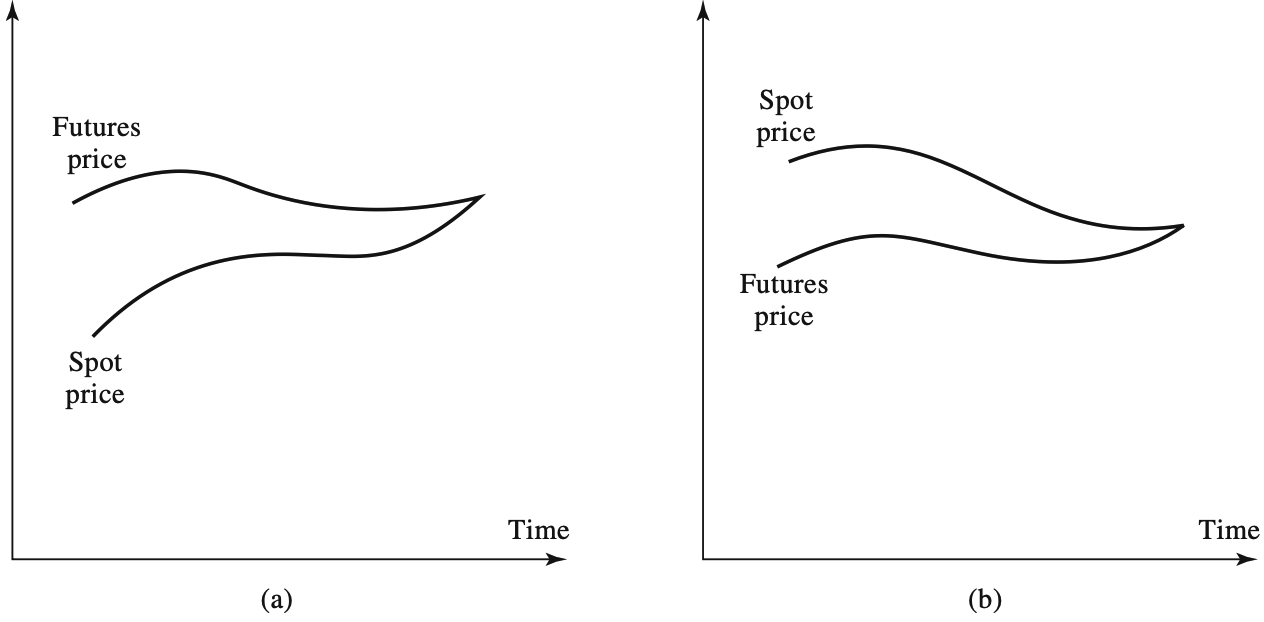
\includegraphics[scale=0.4]{derivatives/convgspotfuture}
\caption{Convergence of futures price to spot price.}
\end{figure}

Suppose futures price is above spot price during delivery period. Traders have clear arbitrage opportunity: short futures, long asset, make delivery. The futures price will then fall.\\
If futures price is below spot price during delivery period, traders will long futures, wait for delivery, and the futures price will then rise.\\

Options are traded both on exchanges and OTC.

\begin{definition} A \hlt{call option} (\hlt{put option}) gives the holder the right to sell (buy) the underlying asset by a certain date for a certain price.
\end{definition}

\begin{definition} An \hlt{American option} can be exercised at any time up to expiration date. An \hlt{European option} can only be exercised on expiration date itself.
\end{definition}

\subsubsection{Clearing House}

Margin accounts are used by exchanges to organise trading so that contract defaults are avoided. \\
Trader has to keep funds in a margin account; the amount to be deposited at the time the contract is entered into is the \hlt{initial margin}. At each of trading day, margin account is adjusted to reflect trader's P\&L (\hlt{daily settlement}, \hlt{marking to market}). Daily settlement leads to funds flowing daily between traders with long positions and traders with short positions; this daily flow of funds to reflect P\&L is the \hlt{variation margin}. Trading via brokers requires a \hlt{maintenance margin}, which is lower than initial margin; if balance in margin account falls below maintenance margin, trader receives \hlt{margin call} and is required to top up to initial margin level within short period of time, or else broker closes out the position. Trader is also entitled to withdraw any balance in margin account that is in excess of the initial margin. Brokers pay interest on balance in margin account.\\
A forward contract is settled at end of life, while futures contract is settled daily. Minimum levels for initial and maintenance margins are set by exchange clearing house. Minimum margin levels are determined by variability of the price of underlying asset, revised when necessary.\\

The clearing house acts as intermediary in futures transactions, and keep track of all daily transactions for calculating net positions of each of its members. Members must provide initial margin reflecting the total number of contracts cleared. The maintenance margin is set equal to initial margin. In determining margin requirements, the number of contracts outstanding is calculated on a net basis rather than a gross basis. Members are required to contribute to a guaranty fund, which is used in the event that a member defaults, and the member's margin is insufficient to cover losses.

\subsubsection{OTC Markets}

OTC markets use central counterparties (CCPs), which perform the same role as exchange clearing houses. Members of CCP provide both initial margin and daily variation margin, and contribute to a guaranty fund. If an OTC derivative transaction has been agreed upon between parties A and B, and CCP accepts the transaction, they become the counterparty to both A and B. CCP hence takes on credit risk of both A and B.\\
Transactions are valued daily, and there are daily variation margin payments between members.\\

For bilaterally cleared OTC, two companies enter a master agreement covering all their trades (ISDA). The agreement includes a credit support annex (CSA), requiring both parties to provide collateral. Collateral agreements in CSAs usually require transactions to be valued daily. Since 2016, regulations require both initial margin and variation margin between financial institutions.

\subsubsection{Interest Rates}

\begin{definition} \hlt{Credit spread} is the difference between the interest rate and risk free rate.
\end{definition}

\hlt{(Treasury Rates)} The rates on Treasury bills and Treasury bonds. The Treasury rates of developed countries are regarded as risk-free rates, as it is assumed that there is no chance the government will default.\\

\hlt{(Overnight Rates)} Borrowing and lending overnight by financial institutions to match asset and liabilities requirements for reserves; the overnight rate is the \hlt{federal funds rate}. The weighted average of rates in brokered transactions is the \hlt{effective federal funds rate}. The Federal Reserve may intervene with its own transactions to raise or lower the rates.\\

\hlt{(Repo Rates)} Secured borrowing rates; the difference between the price at which securities are sold and then repurchased. If structured carefully, involves very little credit risk. Most common type of repo is an \hlt{overnight repo}. In longer term arrangements, \hlt{term repos} are used.\\

The terminal value of an investment $A$ invested at interest rate of $R$ per annum, compounded $m$ times per annum, is $A(1+\frac{R}{m})^{mn}$. If $m=1$, the rate is the \hlt{equivalent annual interest rate}. If continuous compounded is used, then  the terminal value at the end of a year is $Ae^{R}$.\\

The \hlt{$n$-year spot-rate} is the interest rate earned on a zero-coupon bond. The \hlt{Bond Price} is the present value of all cash flows that will be received by owner of the bond, with different spot rate for each cash flow. The \hlt{Bond Yield} is the discount rate that, when applied to all cash flows, gives a bond price equal to its market price. The \hlt{Par Yield} for a certain bond maturity is the coupon rate that causes the bond price to equal its par value.\\

\begin{definition}
\hlt{Forward Rates} are rates implied by current spot rates for periods of time in the future.
\end{definition}

Given $R_1, R_2$ the spot rates for maturities $T_1, T_2$ respectively, and $R_F$ the forward rate between $T_1$ and $T_2$, then
\begin{equation}
R_F = \frac{R_2 T_2 - R_1 T_1}{T_2 - T_1}=R_2 + (R_2 - R_1)\frac{T_1}{T_2 - T_1} \nonumber
\end{equation}
Given the spot rate $R$ for maturity $T$, the \hlt{instantaneous forward rate} for maturity of $T$ is then
\begin{equation}
R_F = R + T \frac{\partial R}{\partial T} \nonumber
\end{equation}
If $P(0,T) = e^{-RT}$ is the price of zero-coupon bond maturity at time $T$, the equation is then
\begin{equation}
R_F = -\frac{\partial}{\partial T} \ln P(0,T) \nonumber
\end{equation}

\begin{definition}
\hlt{Forward Rate Agreement (FRA)} is an agreement to exchange a predetermined rate for a reference rate that will be observed in the market at a future time.
\end{definition}

Let $R_K$ be the fixed rate, $R_F$ be the current forward rate for the reference rate, $\tau$ be the period of time to which the rates apply, $L$ be the principal in the contract.\\
For the party that receives the fix rate, the FRA has a present value of 
\begin{equation}
\tau (R_K - R_F)L \nonumber
\end{equation}
For the party that pays the fix rate, the FRA has a present value of
\begin{equation}
\tau (R_F - R_K)L \nonumber
\end{equation}

\begin{definition}
The \hlt{Duration} of a bond is a measure of how long the holder of the bond has to wait before receiving the present value of the cash payments.
\end{definition}

Let $c_i$ be cash flow at time $t_i$ ($1 \leq i \leq n$). Bond price $B$, yield $y$ (continuously compounded) are related by
\begin{equation}
B = \sum\limits_{i=1}^n c_i e^{-y t_i} \nonumber
\end{equation}
The Duration $D$ of the bond is then
\begin{equation}
D = \sum\limits_{i=1}^n t_i \left[ \frac{c_i e^{-y t_i}}{B} \right] \nonumber
\end{equation}
where the term in square brackets is ratio of present value of cash flow at $t_i$ to bond price. Duration is hence a time-weighted average of the times when payments are made.\\
The relationship between duration and yield is as follows:
\begin{align}
\Delta B &= \frac{dB}{dy} \Delta y \nonumber \\
\frac{\Delta B}{B} &= - D \Delta y \nonumber
\end{align}

If $y$ is expressed with compounding frequency of $m$ times a year, then the relationship becomes
\begin{equation}
\Delta B = - \frac{BD \Delta y}{1 + y/m} \nonumber
\end{equation}
Hence, the \hlt{modified duration} is 
\begin{equation}
D^* = \frac{D}{1 + y/m} \nonumber
\end{equation}
The duration relationship is then
\begin{equation}
\Delta B = - B D^* \Delta y \nonumber
\end{equation}

When duration is used for bond portfolios, it is assumed that the yields of all bonds will change by approximately the same amount, i.e., a parallel shift in the spot yield curve. The portfolio may still be exposed to shifts that are either large or non-parallel.\\
\hlt{Convexity} may be used to improve the relationship in the equation. Convexity is defined as
\begin{equation}
C = \frac{1}{B} \frac{d^2 B}{dy^2} \nonumber
\end{equation}
By Taylor series, we then have the relationship
\begin{equation}
\frac{\Delta B}{B} = -D \Delta y + \frac{1}{2}C(\Delta y)^2 \nonumber
\end{equation}

To determine the underlying reasons for the shape of the spot curve, theories on term structure of interest rates are referred to.\\

\hlt{(Expectations Theory)} A forward interest rate corresponding to a certain future period is equal to the expected future zero interest rate for that period.\\

\hlt{(Market Segmentation Theory)} There exists no relationship between short, medium, and long-term interest rates, as investors do not readily switch from one maturity to another.\\

\hlt{(Liquidity Preference Theory)} Investors prefer to preserve their liquidity and invest funds for short periods of time. Borrowers prefer to borrow at fixed rates for long periods of time. Hence forward rates are greater than expected future spot rates.






\newpage

\subsection{Forwards and Futures}

\subsubsection{Pricing}



\subsubsection{Hedging with Futures}

The fundamentals of hedging with futures are \hlt{hedge-and-forget} strategies, where no changes is made to adjust the hedge once it has been put in place.

\begin{definition}
\hlt{(Basic Principles of Futures Hedging)}\\
The objective is to take a position that neutralises the risk as far as possible.
\begin{enumerate}[label=\roman*.]
\setlength{\itemsep}{0pt}
\item \hlt{Short Hedge}: short position on futures. \\
Used when hedger already owns an asset and will sell the asset at some time in the future; or when asset is not owned right now but will be owned and ready for sale sometime in the future.
\item \hlt{Long Hedge}: long position on futures. \\
Used when hedger will purchase an asset in the future and wants to lock in the price now.
\end{enumerate}
\begin{table}[h]
\begin{tabular}{|c | c | c|}
\hline
 & \textbf{Short Hedge} & \textbf{Long Hedge} \\ \hline
May $15$ & \makecell[l]{Spot: $50$ \\ Futures: $49$} & \makecell[l]{Spot: $50$ \\ Futures: $49$} \\ \hline
August $15$ Scenario 1 & \makecell[l]{Spot: $45$ \\ Gain from hedge: $4$} &  \makecell[l]{Spot: $45$ \\ Loss from hedge: $4$} \\ \hline
August $15$ Scenario 2 & \makecell[l]{Spot: $55$ \\ Loss from hedge: $6$} & \makecell[l]{Spot: $55$ \\ Gain from hedge: $6$} \\ \hline
\end{tabular}
\end{table}
\end{definition}

In practice, hedging is not perfect due to factors as follows:
\begin{enumerate}[label=\arabic*.]
\setlength{\itemsep}{0pt}
\item Asset being hedged is not exactly the same as the asset underlying the futures contract.
\item Uncertainty as to exact date in which the asset will be bought or sold.
\item Hedge may require the futures contract to be closed out before its delivery month.
\end{enumerate}
These lead to \hlt{basis risk}.

\begin{definition}
The \hlt{basis} in a hedging situation is defined as
\begin{align}
\text{Basis} = \text{Spot Price} - \text{Futures Price} \nonumber
\end{align}
An increase/decrease in basis is a strengthening/weakening of the basis.
\end{definition}

\begin{definition}
Let $S_i$ be spot price at time $t_i$, $F_i$ be futures price at time $t_i$, $b_i$ be basis price at time $t_i$.	 Assume hedge is placed at time $t_1$, closed at time $t_2$. Price realised for asset is $S_2$, profit from futures position is $F_1 - F_2$.  Effective price obtained for asset hedging is therefore $S_2 + F_1 - F_2 = F_1 + b_2$.\\
If $b_2$ is known, perfect hedge will result. The \hlt{basis risk} is the hedging risk from uncertainty associated with $b_2$.
\end{definition}

\begin{definition}
\hlt{Cross Hedging} occurs when the asset underlying the futures contract is not the same as the asset whose price is being hedged.
\end{definition}

Cross hedging is often used when futures of the original asset being hedged are not actively traded on the market, and the hedger seeks an alternative asset to hedge the original asset.

\begin{definition}
\hlt{Hedge Ratio} is the ratio of size of position taken in futures contract to the size of exposure.
\end{definition}

Assuming no daily settlement of futures contracts, hedger seeks a hedge ratio that minimises variance of hedged position value. Let $\Delta S$ be change in spot price, $\Delta F$ change in futures price. Assuming linear relationship,
\begin{equation}
\Delta S = a + b \Delta F + \epsilon	 \nonumber
\end{equation}
where $a,b$ are constants, $\epsilon$ is an error term. Suppose hedge ratio is $h$. Change in value of position per unit of exposure to $S$ is:
\begin{equation}
\Delta S - h \Delta F = a + (b-h) \Delta F + \epsilon \nonumber
\end{equation}
Standard deviation is minimised by setting $h=b$. Let minimum variance hedge ratio be $h^*$. Then
\begin{equation}
h^* = \rho \frac{\sigma_S}{\sigma_F} \nonumber
\end{equation}
where $\sigma_S, \sigma_F$ is standard deviation of $\Delta S, \Delta F$ respectively, $\rho$ is coefficient of correlation.

\begin{figure}[H]
\centering
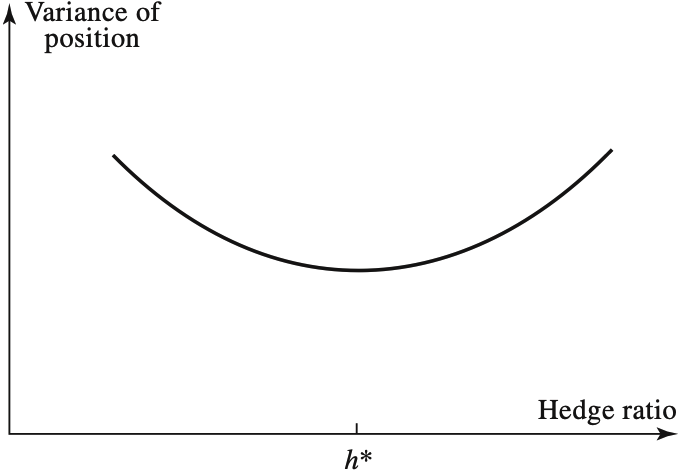
\includegraphics[scale=0.5]{derivatives/hedgeratio}
\caption{Dependence of variance of position on hedge ratio.}
\end{figure}

\hlt{Hedge effectiveness} is the proportion of variance eliminated by hedging. This is $R^2$ from regression of $\Delta S$ against $\Delta F$, and equals $\rho^2$. Parameters $\rho$, $\sigma_S$, $\sigma_F$ are estimated from historical data on $\Delta S$ and $\Delta F$.\\

The optimal number of futures to be used in hedging is
\begin{equation}
N^* = \frac{h^* Q_A}{Q_F} \nonumber
\end{equation}
where $Q_A$ is size of potion being hedged (units), $Q_F$ is size of one futures contract (units). The futures contract should be on $h^* Q_A$ units of the asset.\\

If daily settlement is used, there are a series of one-day hedges, and thus let $\hat{\sigma}_S, \hat{\sigma}_F$ be standard deviation of percentage one-day changes in spot and future price respectively, $\hat{\rho}$ be correlation between percentage one-day changes in spot and future prices. The optimal one day hedge is then
\begin{equation}
h^* = \hat{\rho}\frac{\hat{\sigma}_S S}{\hat{\sigma}_F F} \nonumber
\end{equation} 
and the optimal number of futures to be used is then
\begin{equation}
N^* = \hat{\rho}\frac{\hat{\sigma}_S S Q_A}{\hat{\sigma}_F F Q_F} \nonumber
\end{equation}

If an interest $r\%$ per annum is earned or paid over the remaining life of the hedge, then the optimal number of futures is $N^* / (1+0.01r)$; this is \hlt{tailing the hedge}.\\

Stock index futures may be used to hedge a well diversified equity portfolio. Let $V_A, V_F$ be the current value of portfolio and one futures contract respectively.\\
If portfolio mirrors the index, the optimal hedge ratio is then $1.0$, and number of futures contracts to be shorted is then $N^* = \frac{V_A}{V_F}$. If portfolio do not mirror the index, then capital asset pricing model (CAPM) should be used to determine beta ($\beta$), and the number of futures contracts to be shorted is then $N^* = \beta \frac{V_A}{V_F}$, assuming maturity of futures contract is close to the maturity of the hedge.\\

If instead, the hedger wishes to change the beta of portfolio where $\beta > \beta^*$, a short position $(\beta - \beta^*)\frac{V_A}{V_F}$ is required. If $\beta < \beta^*$, then a long position $(\beta^* - \beta)\frac{V_A}{V_F}$ is required.\\

Stock index hedging is typically used when the portfolio manager is uncertain about performance of market, but is confident that the stocks in the portfolio will outperform the market. The hedger may also be planning to hold a portfolio for a long period of time and requires short-term protection in an uncertain market situation.\\

If expiration date of hedge is later than delivery dates of all futures contracts that may be used, then the hedger may \hlt{stack and roll} by closing out one futures contract and taking the same position in a futures contract with a later delivery date.





\newpage

\newpage

\section{Currency Trading}



\newpage

\section{Commodities Trading}



%{\color{white}space}
%\begin{enumerate}[label=\roman*.]
%\setlength{\itemsep}{0pt}
%\item
%\end{enumerate}

%\raggedright

%\begin{figure}[H]
%\centering
%\includegraphics[scale=0.4]{dihedralgroups}
%\caption{Example of an equilateral triangle as a Dihedral Group $D_6$}
%\end{figure}

\newpage

\bibliography{references}

\end{document}
	